\chapter{RESULT}

To evaluate the performance of the Nepali speech-to-text model, \textbf{Word Error Rate (WER)} was used as the primary evaluation metric. WER is commonly used in speech recognition systems and is calculated as:

\begin{equation}
\text{WER} = \frac{S + D + I}{N}
\end{equation}

where:
\begin{itemize}
    \item $S$ = Substitutions
    \item $D$ = Deletions
    \item $I$ = Insertions
    \item $N$ = Total words in the reference
\end{itemize}

The model was tested on a held-out Nepali audio dataset consisting of conversational and formal speech. The system achieved a \textbf{Average Word Error Rate of 9.22\%}, indicating that approximately one-third of the words were misrecognized. This result suggests that the model has moderate performance, with room for improvement through better data preprocessing, acoustic modeling, or language modeling.
% \begin{figure}[H]  % You can use [h] or [H] with \usepackage{float}
%     \centering
%     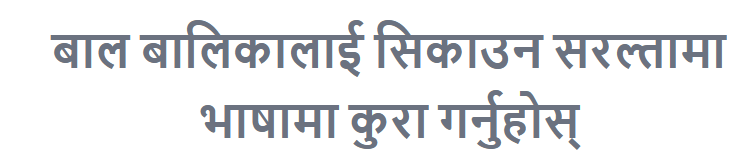
\includegraphics[width = \textwidth]{Images/sentence.png}
%     \caption{Word Error Rate of Different outputs}
%     \label{fig:ref_vs_hyp}
% \end{figure}



% for MA BIHANAI UTHERA CLZ JANXU
\begin{figure}[H]  % You can use [h] or [H] with \usepackage{float}
    \centering
    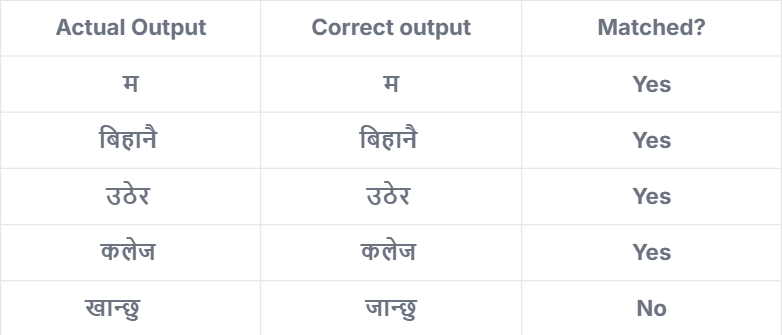
\includegraphics[width=\textwidth]{Images/eg1.png}
    \caption{Comparison between Reference and Hypothesis Outputs with error }
    \label{fig:ref_vs_hyp}
\end{figure}
\text{}\\
Substitution (S) = 1 \\
Deletion (D) = 0 \\
Insertion (I) = 0 \\
Total number of words in reference (N) = 5 \\



\begin{equation}
\text{WER} = \frac{S + D + I}{N}\\
\end{equation}

\begin{equation}
\text{WER} = \frac{1 + 0 + 0}{5} = \frac{1}{5} = 0.2\\
\end{equation}

\text{So we got the}
 \textbf{Word Error Rate (WER)} = \textbf{0.2}(20\%) for this sentence \\








\section{Reference vs Hypothesis Outputs}

\begin{figure}[H]  % You can use [h] or [H] with \usepackage{float}
    \centering
    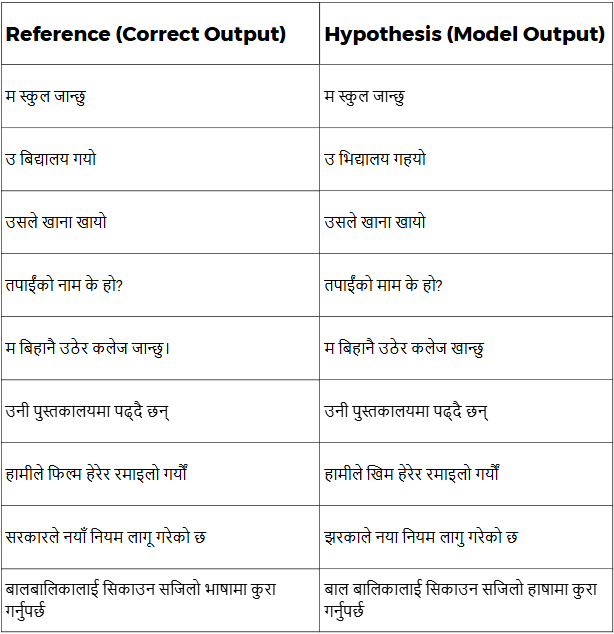
\includegraphics[width=\textwidth]{Images/output.png}
    \caption{Comparison between Reference and Hypothesis Outputs}
    \label{fig:ref_vs_hyp}
\end{figure}








%start


\begin{figure}[H]  % You can use [h] or [H] with \usepackage{float}
    \centering
    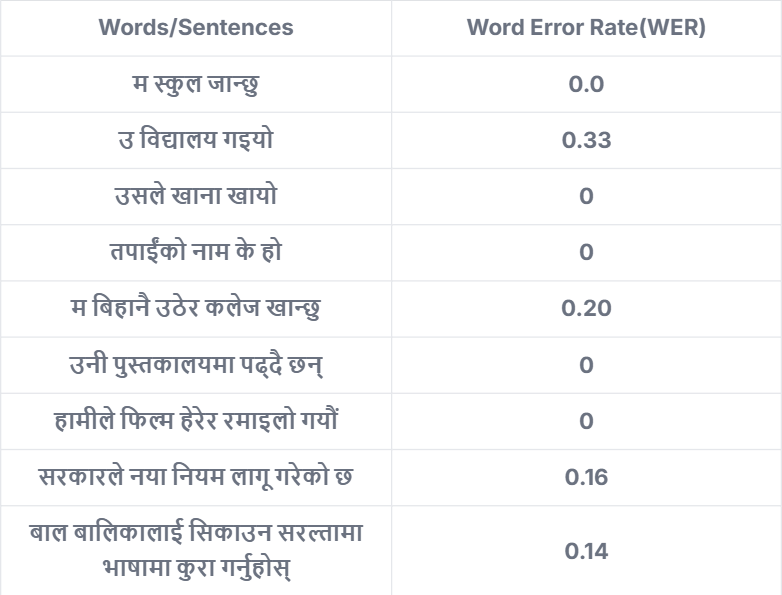
\includegraphics[width=\textwidth]{Images/error.png}
    \caption{Word Error Rate of Different outputs}
    \label{fig:ref_vs_hyp}
\end{figure}


\begin{figure}[H]  % You can use [h] or [H] with \usepackage{float}
    \centering
    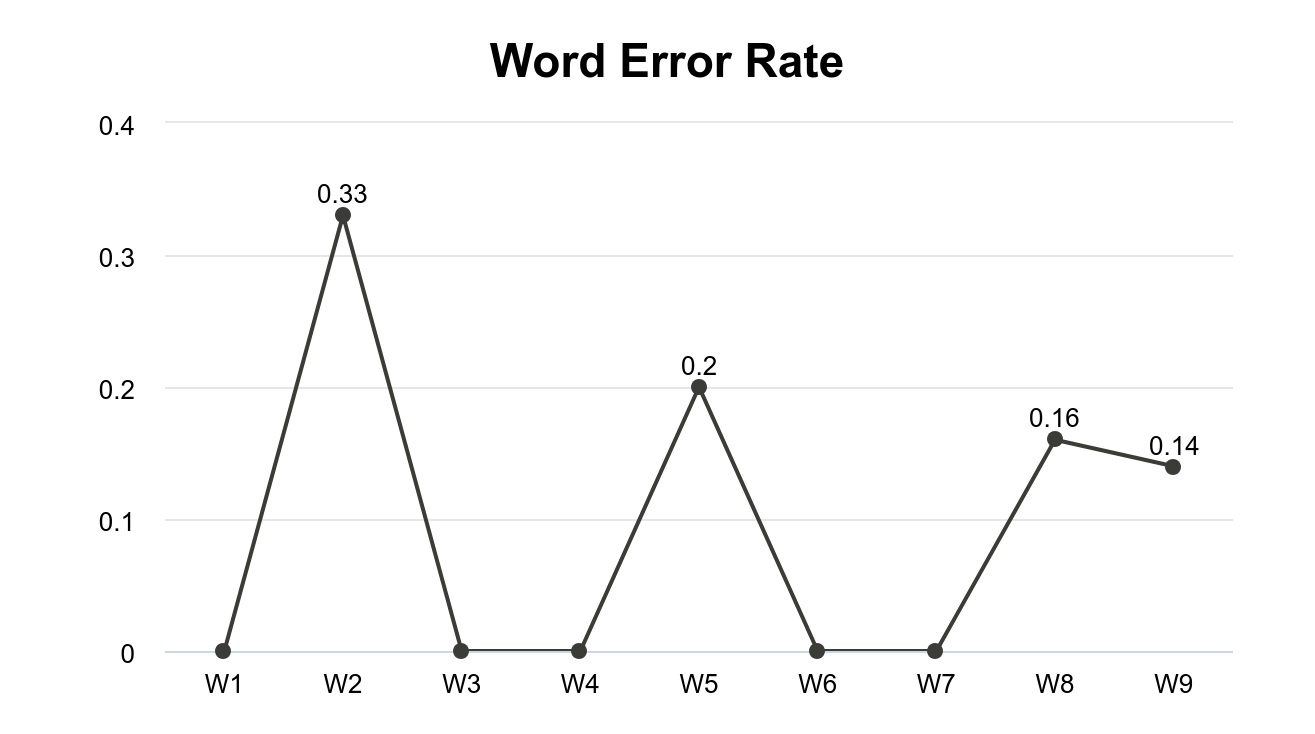
\includegraphics[width=\textwidth]{Images/graph.png}
    \caption{Graph of Word Error Rate of different outputs}
    \label{fig:ref_vs_hyp}
\end{figure}


%end







 

% \begin{figure}[H]  % You can use [h] or [H] with \usepackage{float}
%     \centering
%     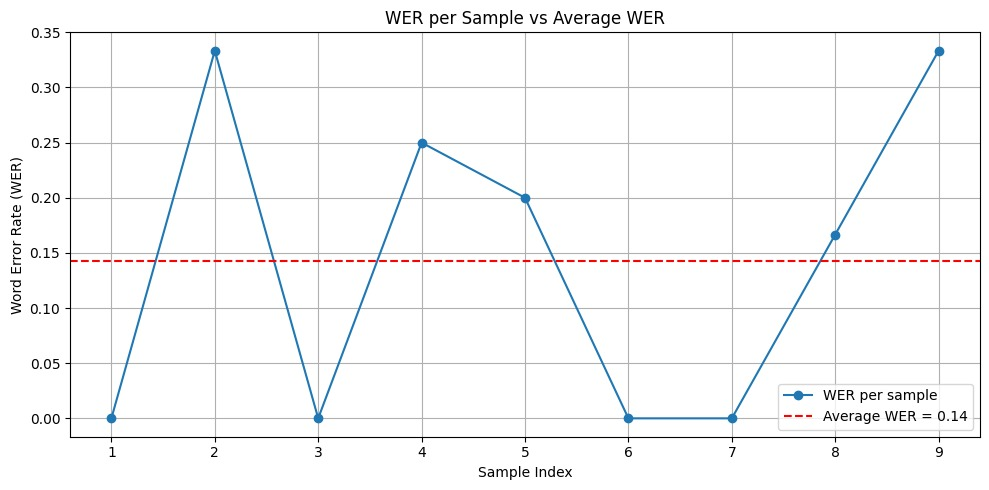
\includegraphics[width=\textwidth]{Images/wer.jpg}
%     \caption{Word error rate}
%     \label{fig:word_error_rate}
% \end{figure}

\begin{figure}[H]  % You can use [h] or [H] with \usepackage{float}
    \centering
    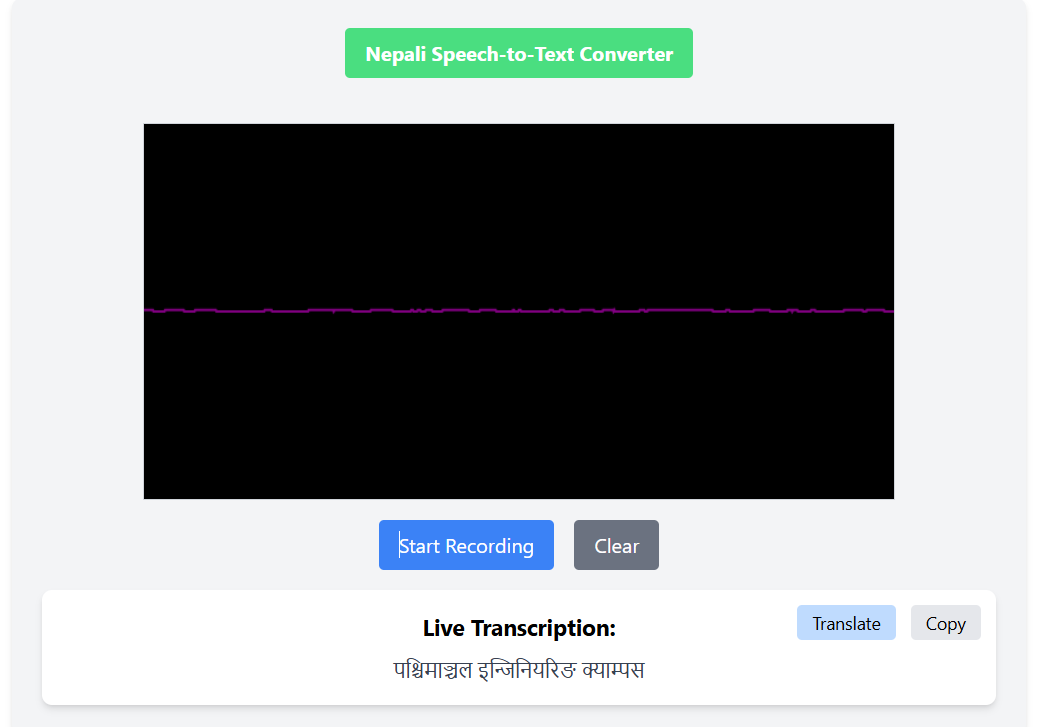
\includegraphics[width=\textwidth]{Images/op1-after.png}
    \caption{Output 1}
    \label{fig:ref_vs_hyp}
\end{figure}


\begin{figure}[H]  % You can use [h] or [H] with \usepackage{float}
    \centering
    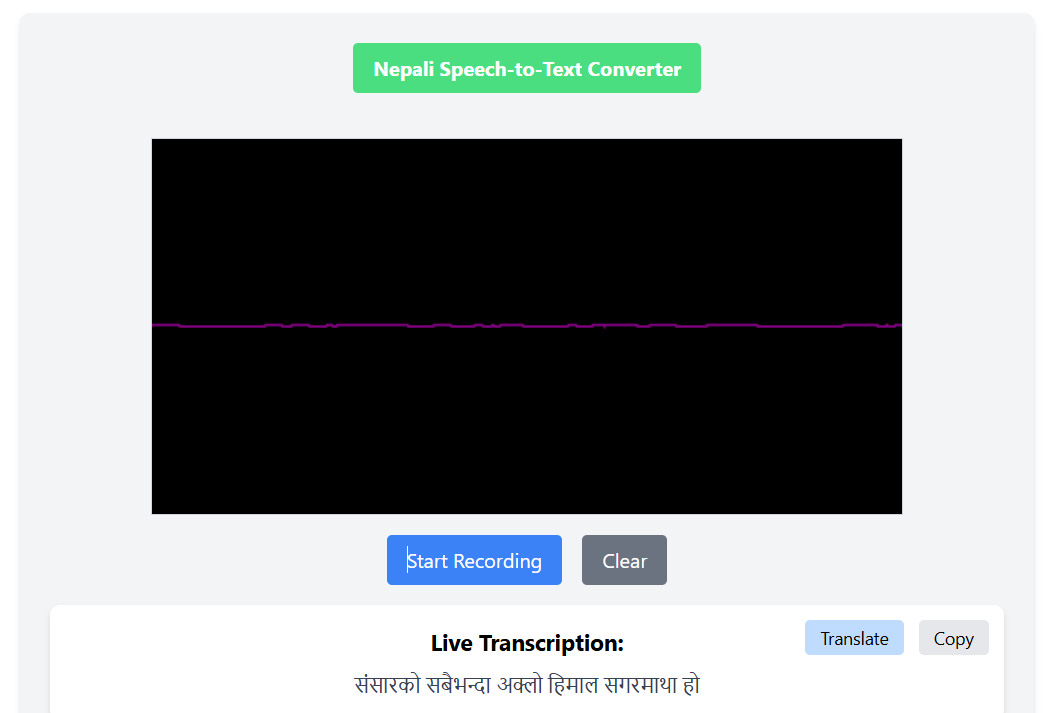
\includegraphics[width=\textwidth]{Images/op2-after.png}
    \caption{Output 2}
    \label{fig:ref_vs_hyp}
\end{figure}


